\documentclass{beamer}\usepackage[]{graphicx}\usepackage[]{color}
%% maxwidth is the original width if it is less than linewidth
%% otherwise use linewidth (to make sure the graphics do not exceed the margin)
\makeatletter
\def\maxwidth{ %
  \ifdim\Gin@nat@width>\linewidth
    \linewidth
  \else
    \Gin@nat@width
  \fi
}
\makeatother

\definecolor{fgcolor}{rgb}{0, 0, 0}
\newcommand{\hlnum}[1]{\textcolor[rgb]{0.533,0,0.133}{#1}}%
\newcommand{\hlstr}[1]{\textcolor[rgb]{0.667,0.267,0}{#1}}%
\newcommand{\hlcom}[1]{\textcolor[rgb]{1,0.533,0}{#1}}%
\newcommand{\hlopt}[1]{\textcolor[rgb]{0,0,0}{\textbf{#1}}}%
\newcommand{\hlstd}[1]{\textcolor[rgb]{0,0,0}{#1}}%
\newcommand{\hlkwa}[1]{\textcolor[rgb]{0.4,0.067,0.067}{\textbf{#1}}}%
\newcommand{\hlkwb}[1]{\textcolor[rgb]{0,0,0.4}{\textbf{#1}}}%
\newcommand{\hlkwc}[1]{\textcolor[rgb]{0,0,0.4}{#1}}%
\newcommand{\hlkwd}[1]{\textcolor[rgb]{0,0.267,0.4}{#1}}%
\let\hlipl\hlkwb

\usepackage{framed}
\makeatletter
\newenvironment{kframe}{%
 \def\at@end@of@kframe{}%
 \ifinner\ifhmode%
  \def\at@end@of@kframe{\end{minipage}}%
  \begin{minipage}{\columnwidth}%
 \fi\fi%
 \def\FrameCommand##1{\hskip\@totalleftmargin \hskip-\fboxsep
 \colorbox{shadecolor}{##1}\hskip-\fboxsep
     % There is no \\@totalrightmargin, so:
     \hskip-\linewidth \hskip-\@totalleftmargin \hskip\columnwidth}%
 \MakeFramed {\advance\hsize-\width
   \@totalleftmargin\z@ \linewidth\hsize
   \@setminipage}}%
 {\par\unskip\endMakeFramed%
 \at@end@of@kframe}
\makeatother

\definecolor{shadecolor}{rgb}{.97, .97, .97}
\definecolor{messagecolor}{rgb}{0, 0, 0}
\definecolor{warningcolor}{rgb}{1, 0, 1}
\definecolor{errorcolor}{rgb}{1, 0, 0}
\newenvironment{knitrout}{}{} % an empty environment to be redefined in TeX

\usepackage{alltt}
\newenvironment{changemargin}[2]{%
\begin{list}{}{%
\setlength{\topsep}{0pt}%
\setlength{\leftmargin}{#1}%
\setlength{\rightmargin}{#2}%
\setlength{\listparindent}{\parindent}%
\setlength{\itemindent}{\parindent}%
\setlength{\parsep}{\parskip}%
}%
\item[]}{\end{list}}
\usepackage{graphicx}
\usepackage{amsmath}
\usepackage{url}
\usetheme{Madrid}
\usecolortheme{beaver}
\setbeamertemplate{navigation symbols}{}
\titlegraphic{
\includegraphics[width=5cm]{..//..//S-DS-VC-RGB.png}}
%\logo{
\includegraphics[width=0.1\textwidth,keepaspectratio]{..//..//UOACrest.png}}
\author[SCC]{Statistical Consulting Centre}%\\
\institute[\href{mailto:consulting@stat.auckland.ac.nz}
  {consulting@stat.auckland.ac.nz}]{\href{mailto:consulting@stat.auckland.ac.nz}
  {consulting@stat.auckland.ac.nz}\\
%Statistical Consulting Centre\\
The Department of Statistics\\
The University of Auckland}
\title[Session 2 -- Subsetting data]{NZSSN Courses: Introduction to \texttt{R}}
\subtitle{Session 2 -- Subsetting data} 
\date{1 March, 2017}
\IfFileExists{upquote.sty}{\usepackage{upquote}}{}
\begin{document}
\maketitle
\begin{frame}
\vspace{10pt}
  \frametitle{Functions}
  A function is a relationship between a set of inputs (arguments)
    and a set of outputs. E.g., the function is fed some information on which it
    operates, the results of which are the output.
    

\vspace{-60pt}
\begin{figure}[h]
  \centering
  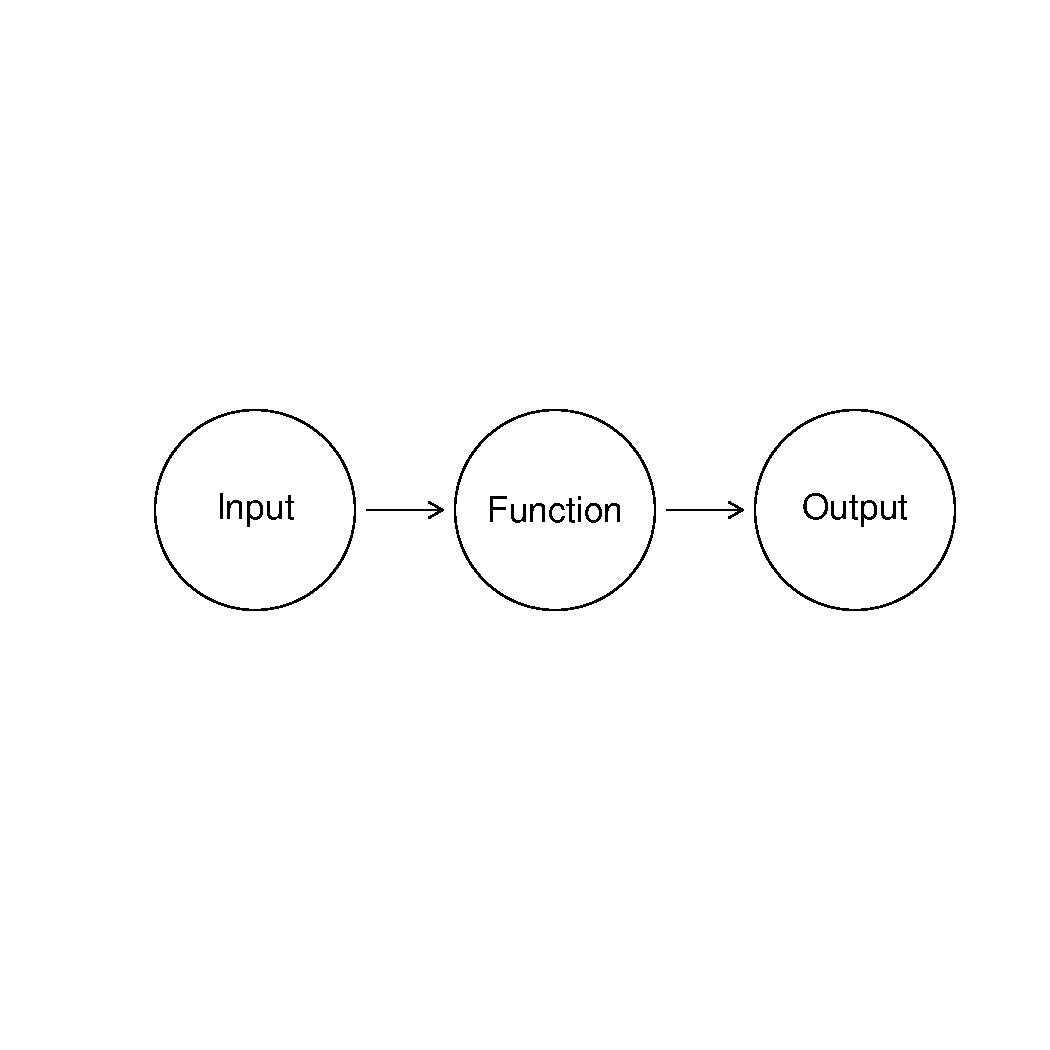
\includegraphics[height = 0.9\textwidth, keepaspectratio]{Figure/fun1}
  \label{fig:fun1}
\end{figure}

This is an essential building block for the R package. 

\end{frame}

\begin{frame}
  \frametitle{Functions}
\vspace{10pt}
  We have seen many functions, e.g. \texttt{log},
    \texttt{mean}, \texttt{table}, \texttt{with}, etc.

\vspace{-60pt}
\begin{figure}[h]
  \centering
  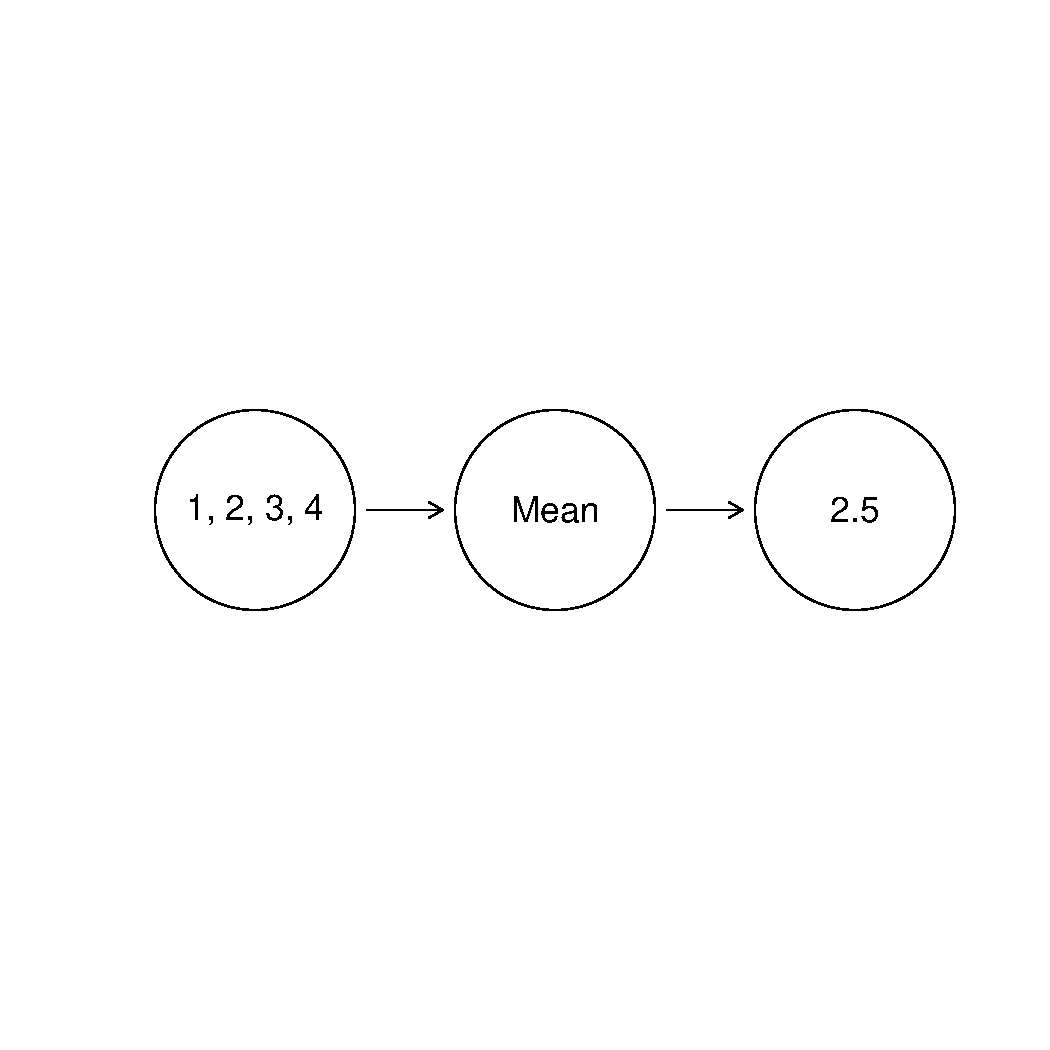
\includegraphics[height = 0.9\textwidth, keepaspectratio]{Figure/fun2}
  \label{fig:fun2}
\end{figure}
\end{frame}

\begin{frame}[fragile]
  \frametitle{Working with functions}
\begin{itemize}
   \item Functions can be user-defined, i.e., you can write your own.
   \item Output is the last line of the function. You can use \texttt{return()} to specifiy the output.
   \item Here is a function calculates the standard error of the mean (SEM).
\end{itemize}

\begin{knitrout}
\definecolor{shadecolor}{rgb}{0.965, 0.965, 0.965}\color{fgcolor}\begin{kframe}
\begin{alltt}
\hlstd{mystder} \hlkwb{<-} \hlkwa{function}\hlstd{(}\hlkwc{x}\hlstd{)\{}
    \hlstd{mysd} \hlkwb{<-} \hlkwd{sd}\hlstd{(x,} \hlkwc{na.rm} \hlstd{=} \hlnum{TRUE}\hlstd{)} \hlcom{# Calc std. deviation}
    \hlstd{n} \hlkwb{<-} \hlkwd{length}\hlstd{(x)}              \hlcom{# Calc sample size}
    \hlstd{mysd}\hlopt{/}\hlkwd{sqrt}\hlstd{(n)}                \hlcom{# Definition of SEM}
\hlstd{\}}
\hlkwd{mystder}\hlstd{(issp.df}\hlopt{$}\hlstd{Age)}
\end{alltt}
\begin{verbatim}
[1] 0.5101842
\end{verbatim}
\end{kframe}
\end{knitrout}
\begin{itemize}
  \item A set of user-defined functions can be bundled together into an R \texttt{package}.
\end{itemize}
\end{frame}


\begin{frame}[fragile]
  \frametitle{Getting data into \texttt{R}}
\begin{itemize}
  \item Base \texttt{R} includes only functions which read data sets saved in simple file formats, e.g. \texttt{csv}, \texttt{txt}, tab delimited, etc.
  \item What if your data was saved in another format, e.g. STATA, SPSS, or SAS spreadsheets? 
  \item The \texttt{haven} package for \texttt{R} contains functions that may help!
  \url{https://cran.r-project.org/web/packages/haven/index.html}
\end{itemize}
%\begin{alltt}
\begin{verbatim}
> library(haven)
> stata <- read_dta("data.dta")
> spss <- read_sav("data.sav")
> sas <- read_sas("data.sas7bdat")
> sasxport <- read_xpt("data.xpt")
\end{verbatim}
%\end{alltt}
However, it is always the easiest and safest to read data into \texttt{R} from a \texttt{csv} file.
\end{frame}

\begin{frame}
  \frametitle{Packages}
  \begin{itemize}
  \item Currently, the CRAN package repository features 10,098 available
    packages (17 Feb. 2017). There are about 12,383 CRAN, BioConductor and Github packages in total.
  \item To install packages from the \texttt{R} GUI, click on
    \texttt{Packages} $\rightarrow$ \texttt{Install Package(s) ...}
    $\rightarrow$ \texttt{New Zealand (or whatever region you are
    located)} $\rightarrow$ \texttt{Package name}
  \item Or, you can type \texttt{install.packages("\textit{package name}")}, e.g. \texttt{install.packages("haven")}. 
  \item After the installation, use  \texttt{library(\textit{package name})}
        to load it into \texttt{R}. Note: Installation is performed only once; however,
        it must be loaded (i.e. use the command \texttt{library(\textit{package name})})
        in \emph{every} \texttt{R} session.
  \end{itemize}
\end{frame}


\begin{frame}[fragile]
  \frametitle{Two-way frequency tables}
\begin{knitrout}
\definecolor{shadecolor}{rgb}{0.965, 0.965, 0.965}\color{fgcolor}\begin{kframe}
\begin{alltt}
\hlstd{income.gender.tab} \hlkwb{<-} \hlkwd{with}\hlstd{(issp.df,}
                          \hlkwd{table}\hlstd{(Income, Gender))}
\hlstd{income.gender.tab}
\end{alltt}
\begin{verbatim}
                        Gender
Income                   Female Male NA, refused
  $10000 or less            177   57           4
  $10001-$15000             115   35           2
  $15001-$20000              49   29           2
  $20001-$25000              65   50           0
  $25001-$30000              71   48           2
  $30001-$40000              59   70           4
  $40001-$50000              27   47           2
  $50001-$70000               7   27           1
  $70001-$100000              4   35           2
  NAV; NAP No own income     33   20           3
\end{verbatim}
\end{kframe}
\end{knitrout}
\end{frame}

\begin{frame}[fragile]
  \frametitle{Two-way frequency tables}
  We can convert the counts to percentages, i.e.
\begin{knitrout}
\definecolor{shadecolor}{rgb}{0.965, 0.965, 0.965}\color{fgcolor}\begin{kframe}
\begin{alltt}
\hlkwd{round}\hlstd{(}\hlkwd{prop.table}\hlstd{(income.gender.tab,} \hlnum{2}\hlstd{)} \hlopt{*} \hlnum{100}\hlstd{,} \hlnum{1}\hlstd{)}
\end{alltt}
\begin{verbatim}
                        Gender
Income                   Female Male NA, refused
  $10000 or less           29.2 13.6        18.2
  $10001-$15000            18.9  8.4         9.1
  $15001-$20000             8.1  6.9         9.1
  $20001-$25000            10.7 12.0         0.0
  $25001-$30000            11.7 11.5         9.1
  $30001-$40000             9.7 16.7        18.2
  $40001-$50000             4.4 11.2         9.1
  $50001-$70000             1.2  6.5         4.5
  $70001-$100000            0.7  8.4         9.1
  NAV; NAP No own income    5.4  4.8        13.6
\end{verbatim}
\end{kframe}
\end{knitrout}
\end{frame}

\begin{frame}[fragile]
\frametitle{\texttt{which} Income is unavailable or none?}
Let's use \texttt{R}'s powerful subsetting capabilities to select those cases for which the value of Income is ``NAV; NAP No own income''.

\begin{knitrout}
\definecolor{shadecolor}{rgb}{0.965, 0.965, 0.965}\color{fgcolor}\begin{kframe}
\begin{alltt}
\hlstd{index} \hlkwb{<-} \hlkwd{which}\hlstd{(issp.df}\hlopt{$}\hlstd{Income}
               \hlopt{==} \hlstr{"NAV; NAP No own income"}\hlstd{)}
\hlstd{index}
\end{alltt}
\begin{verbatim}
 [1]    9   13   19   22   27   37   77  122  132
[10]  133  141  148  186  197  207  221  222  239
[19]  242  277  283  310  345  354  362  382  383
[28]  390  404  416  438  444  454  463  480  482
[37]  537  551  569  608  629  640  650  758  806
[46]  821  891  910  934  939  944  977  984  986
[55] 1027 1042
\end{verbatim}
\end{kframe}
\end{knitrout}
\end{frame}

\begin{frame}[fragile]
\frametitle{How many are there?}

\begin{knitrout}
\definecolor{shadecolor}{rgb}{0.965, 0.965, 0.965}\color{fgcolor}\begin{kframe}
\begin{alltt}
\hlcom{# Use length() to count the number of elements in "index".}
\hlkwd{length}\hlstd{(index)}
\end{alltt}
\begin{verbatim}
[1] 56
\end{verbatim}
\end{kframe}
\end{knitrout}
\end{frame}

\begin{frame}[fragile]
\frametitle{Who are they?}

\begin{knitrout}
\definecolor{shadecolor}{rgb}{0.965, 0.965, 0.965}\color{fgcolor}\begin{kframe}
\begin{alltt}
\hlcom{# Use square brackets to extract IDs corresponding  }
\hlcom{# to the cases numbers contained in "index"}
\hlstd{issp.df}\hlopt{$}\hlstd{ID[index]}
\end{alltt}
\begin{verbatim}
 [1] 1900097 1900139 1900181 1900205 1900241 1900331
 [7] 1900667 1901345 1901435 1901441 1901531 1901597
[13] 1901028 1901118 1901202 1901328 1901346 1901490
[19] 1901568 1900668 1900578 1900110 1900033 1900129
[25] 1900189 1900435 1900441 1900501 1900675 1900795
[31] 1900981 1901059 1901155 1901227 1901359 1901395
[37] 1900226 1900358 1900562 1900946 1901126 1901234
[43] 1901318 1900647 1901151 1901295 1900372 1900600
[49] 1900888 1900936 1900984 1901290 1901344 1901362
[55] 1900464 1901475
\end{verbatim}
\end{kframe}
\end{knitrout}
\end{frame}

\begin{frame}[fragile]
\frametitle{Subsetting}
Square brackets \texttt{[]} are used to extract subsets of data.
\begin{knitrout}
\definecolor{shadecolor}{rgb}{0.965, 0.965, 0.965}\color{fgcolor}\begin{kframe}
\begin{alltt}
\hlcom{# First element only}
\hlstd{issp.df}\hlopt{$}\hlstd{Gender[}\hlnum{1}\hlstd{]}
\end{alltt}
\begin{verbatim}
[1] "Female"
\end{verbatim}
\begin{alltt}
\hlcom{# All but the first element}
\hlstd{issp.df}\hlopt{$}\hlstd{Gender[}\hlopt{-}\hlnum{1}\hlstd{]}
\end{alltt}
\begin{verbatim}
   [1] "Male"        "Female"      "Female"     
   [4] "Female"      "Male"        "Female"     
   [7] "Male"        "NA, refused" "Male"       
  [10] "Female"      "Female"      "Female"     
  [13] "Female"      "Female"      "Male"       
  [16] "Female"      "Female"      "Male"       
  [19] "Female"      "Female"      "Male"       
  [22] "Female"      "Female"      "Female"     
  [25] "Female"      "Female"      "Female"     
  [28] "Male"        "Male"        "NA, refused"
  [31] "Male"        "Female"      "Female"     
  [34] "Male"        "Female"      "Male"       
  [37] "Female"      "Male"        "Female"     
  [40] "Female"      "Female"      "Female"     
  [43] "Male"        "Male"        "Female"     
  [46] "Female"      "Male"        "NA, refused"
  [49] "Male"        "Female"      "Male"       
  [52] "Female"      "Male"        "Male"       
  [55] "Female"      "Female"      "Male"       
  [58] "Female"      "Male"        "Female"     
  [61] "Male"        "Female"      "Female"     
  [64] "Female"      "Female"      "Female"     
  [67] "Male"        "Male"        "Female"     
  [70] "Male"        "NA, refused" "Female"     
  [73] "Female"      "Female"      "Male"       
  [76] "Female"      "Male"        "NA, refused"
  [79] "Male"        "Female"      "Female"     
  [82] "Male"        "Female"      "Female"     
  [85] "Male"        "Male"        "Female"     
  [88] "Male"        "Female"      "Female"     
  [91] "Male"        "Male"        "Female"     
  [94] "Female"      "Female"      "Female"     
  [97] "NA, refused" "Female"      "Male"       
 [100] "Female"      "Female"      "Female"     
 [103] "Female"      "Male"        "Male"       
 [106] "Female"      "Female"      "Female"     
 [109] "Male"        "Female"      "Male"       
 [112] "Male"        "Female"      "Male"       
 [115] "Female"      "Female"      "Male"       
 [118] "Female"      "Male"        "Female"     
 [121] "Female"      "Female"      "Female"     
 [124] "Male"        "Male"        "Female"     
 [127] "Female"      "Male"        "Male"       
 [130] "Male"        "Male"        "Male"       
 [133] "Female"      "Female"      "Female"     
 [136] "Female"      "Male"        "Female"     
 [139] "Female"      "NA, refused" "Female"     
 [142] "Female"      "Male"        "Male"       
 [145] "Male"        "Male"        "Male"       
 [148] "Male"        "Male"        "Male"       
 [151] "Female"      "Female"      "Male"       
 [154] "Female"      "Male"        "Female"     
 [157] "Male"        "Female"      "Male"       
 [160] "Female"      "Female"      "Male"       
 [163] "Male"        "Male"        "Male"       
 [166] "Female"      "Female"      "Female"     
 [169] "Female"      "Female"      "Male"       
 [172] "Female"      "Female"      "Female"     
 [175] "Male"        "Male"        "Female"     
 [178] "Male"        "Female"      "Female"     
 [181] "Female"      "Female"      "Female"     
 [184] "Female"      "Female"      "Female"     
 [187] "Female"      "Female"      "Male"       
 [190] "Female"      "Female"      "Female"     
 [193] "Female"      "Male"        "Male"       
 [196] "Male"        "Female"      "Female"     
 [199] "Female"      "Female"      "Female"     
 [202] "Male"        "Female"      "Female"     
 [205] "Female"      "Male"        "Female"     
 [208] "Female"      "Male"        "Male"       
 [211] "Male"        "Female"      "Male"       
 [214] "Female"      "Female"      "Female"     
 [217] "Female"      "Female"      "Female"     
 [220] "Female"      "Male"        "Male"       
 [223] "Male"        "Female"      "NA, refused"
 [226] "Female"      "Female"      "Female"     
 [229] "Female"      "Male"        "Female"     
 [232] "Male"        "Female"      "Female"     
 [235] "Female"      "Male"        "Female"     
 [238] "Female"      "Male"        "Male"       
 [241] "Female"      "Female"      "Female"     
 [244] "Male"        "Male"        "Male"       
 [247] "Male"        "Female"      "Male"       
 [250] "Male"        "Male"        "Male"       
 [253] "Female"      "Female"      "Female"     
 [256] "Female"      "Female"      "Female"     
 [259] "Male"        "Male"        "Female"     
 [262] "Female"      "Male"        "Female"     
 [265] "Female"      "Female"      "Male"       
 [268] "NA, refused" "Female"      "NA, refused"
 [271] "Male"        "Female"      "Female"     
 [274] "Male"        "Female"      "Male"       
 [277] "Male"        "Female"      "Female"     
 [280] "Male"        "Female"      "Female"     
 [283] "Male"        "Male"        "Male"       
 [286] "Female"      "Male"        "Female"     
 [289] "Male"        "Female"      "Female"     
 [292] "Male"        "Female"      "Female"     
 [295] "Male"        "Male"        "Female"     
 [298] "Female"      "Female"      "Female"     
 [301] "Male"        "Female"      "Female"     
 [304] "Male"        "Female"      "Female"     
 [307] "Female"      "Male"        "Female"     
 [310] "Female"      "Female"      "Male"       
 [313] "Female"      "Male"        "Female"     
 [316] "Female"      "Male"        "Female"     
 [319] "Male"        "Male"        "Male"       
 [322] "Male"        "Male"        "Female"     
 [325] "Male"        "Female"      "Male"       
 [328] "Female"      "Female"      "Male"       
 [331] "Female"      "Female"      "Female"     
 [334] "Male"        "Male"        "Female"     
 [337] "Female"      "Female"      "Male"       
 [340] "Male"        "Male"        "Male"       
 [343] "Female"      "Male"        "Female"     
 [346] "Female"      "Female"      "Male"       
 [349] "Female"      "Female"      "Male"       
 [352] "Male"        "Female"      "Female"     
 [355] "Female"      "Female"      "Male"       
 [358] "Female"      "Female"      "Female"     
 [361] "Female"      "Female"      "Female"     
 [364] "Female"      "Female"      "Female"     
 [367] "Male"        "Male"        "Female"     
 [370] "Female"      "Male"        "Female"     
 [373] "Female"      "Male"        "Female"     
 [376] "NA, refused" "Male"        "Female"     
 [379] "Male"        "Female"      "NA, refused"
 [382] "Female"      "Male"        "Female"     
 [385] "Male"        "Female"      "Female"     
 [388] "Male"        "Female"      "Female"     
 [391] "Male"        "Female"      "Female"     
 [394] "Male"        "Male"        "Male"       
 [397] "Male"        "Male"        "Male"       
 [400] "Female"      "Female"      "Female"     
 [403] "Female"      "Male"        "Female"     
 [406] "Female"      "Female"      "Female"     
 [409] "Female"      "Female"      "Male"       
 [412] "Male"        "Female"      "Male"       
 [415] "Male"        "Male"        "Female"     
 [418] "Female"      "Female"      "Female"     
 [421] "Female"      "Female"      "Female"     
 [424] "Female"      "Female"      "Male"       
 [427] "Female"      "Female"      "Female"     
 [430] "Female"      "Female"      "Male"       
 [433] "Female"      "Female"      "Male"       
 [436] "Female"      "Male"        "Female"     
 [439] "Female"      "Female"      "Female"     
 [442] "Male"        "Female"      "Female"     
 [445] "Male"        "Male"        "Female"     
 [448] "Male"        "Female"      "Male"       
 [451] "Male"        "Male"        "Male"       
 [454] "Female"      "Female"      "Male"       
 [457] "Female"      "Male"        "Male"       
 [460] "Male"        "Female"      "Male"       
 [463] "Female"      "Male"        "Male"       
 [466] "Male"        "Female"      "Female"     
 [469] "Female"      "Male"        "Male"       
 [472] "Male"        "Female"      "Female"     
 [475] "Female"      "Female"      "Female"     
 [478] "Female"      "Female"      "Female"     
 [481] "Female"      "Female"      "Female"     
 [484] "Male"        "Female"      "Male"       
 [487] "Male"        "Female"      "Female"     
 [490] "Male"        "Male"        "Male"       
 [493] "Male"        "Male"        "Female"     
 [496] "Male"        "Female"      "Male"       
 [499] "Male"        "Male"        "Female"     
 [502] "Male"        "Female"      "Female"     
 [505] "Male"        "Male"        "Female"     
 [508] "Female"      "Female"      "Male"       
 [511] "Female"      "Male"        "Female"     
 [514] "Female"      "Female"      "Female"     
 [517] "Female"      "Female"      "Female"     
 [520] "Female"      "NA, refused" "Male"       
 [523] "Male"        "Male"        "Female"     
 [526] "Female"      "Male"        "Male"       
 [529] "Female"      "Female"      "Male"       
 [532] "Female"      "Female"      "Female"     
 [535] "Female"      "Female"      "NA, refused"
 [538] "Female"      "NA, refused" "Female"     
 [541] "Female"      "Female"      "Male"       
 [544] "Female"      "Female"      "Female"     
 [547] "Female"      "Female"      "Female"     
 [550] "Female"      "Male"        "Female"     
 [553] "Male"        "Female"      "Male"       
 [556] "Female"      "Male"        "Female"     
 [559] "Male"        "Female"      "Male"       
 [562] "Male"        "Female"      "Female"     
 [565] "Male"        "Female"      "Female"     
 [568] "Female"      "Female"      "Female"     
 [571] "Male"        "Female"      "Male"       
 [574] "Female"      "Female"      "Female"     
 [577] "Female"      "Female"      "Male"       
 [580] "Male"        "Male"        "Male"       
 [583] "Female"      "Female"      "Male"       
 [586] "Male"        "Female"      "Male"       
 [589] "Male"        "Male"        "Male"       
 [592] "Male"        "Female"      "Female"     
 [595] "Male"        "Female"      "Male"       
 [598] "Female"      "Female"      "Male"       
 [601] "Female"      "Female"      "Male"       
 [604] "Male"        "Male"        "Female"     
 [607] "Male"        "Male"        "Male"       
 [610] "Male"        "Male"        "Male"       
 [613] "Female"      "Female"      "Female"     
 [616] "Male"        "Female"      "Male"       
 [619] "Female"      "Female"      "Female"     
 [622] "Female"      "Female"      "Female"     
 [625] "Female"      "Female"      "Male"       
 [628] "Female"      "Female"      "Male"       
 [631] "Male"        "Male"        "Female"     
 [634] "Female"      "Male"        "Female"     
 [637] "Male"        "Female"      "Female"     
 [640] "Female"      "Female"      "Male"       
 [643] "Male"        "Female"      "Female"     
 [646] "Female"      "Female"      "Female"     
 [649] "Female"      "Female"      "Female"     
 [652] "Male"        "Female"      "Male"       
 [655] "Male"        "Female"      "Male"       
 [658] "Female"      "Female"      "Male"       
 [661] "Female"      "Male"        "Male"       
 [664] "Female"      "Female"      "Female"     
 [667] "Female"      "Male"        "Male"       
 [670] "Male"        "Male"        "Female"     
 [673] "Female"      "Female"      "Male"       
 [676] "Male"        "Male"        "Female"     
 [679] "Male"        "Female"      "Male"       
 [682] "Female"      "Female"      "Male"       
 [685] "Male"        "Male"        "Male"       
 [688] "Female"      "Female"      "Male"       
 [691] "Male"        "Female"      "Male"       
 [694] "Female"      "Male"        "Female"     
 [697] "Female"      "Female"      "Male"       
 [700] "Male"        "Male"        "Male"       
 [703] "Male"        "NA, refused" "Female"     
 [706] "Female"      "Female"      "Female"     
 [709] "Female"      "Male"        "Male"       
 [712] "Female"      "Female"      "Male"       
 [715] "Male"        "Male"        "Female"     
 [718] "Female"      "Female"      "Female"     
 [721] "Male"        "Female"      "Female"     
 [724] "Female"      "Female"      "Female"     
 [727] "Male"        "Female"      "Female"     
 [730] "Female"      "Female"      "Male"       
 [733] "Female"      "Male"        "Female"     
 [736] "Male"        "Male"        "Male"       
 [739] "Female"      "Male"        "Male"       
 [742] "Female"      "Female"      "Female"     
 [745] "Female"      "Male"        "Female"     
 [748] "Female"      "Male"        "Female"     
 [751] "Female"      "Female"      "Male"       
 [754] "Female"      "Female"      "Female"     
 [757] "Male"        "NA, refused" "NA, refused"
 [760] "Male"        "Male"        "Female"     
 [763] "Female"      "Male"        "Female"     
 [766] "Female"      "Male"        "Male"       
 [769] "Male"        "Female"      "Male"       
 [772] "Female"      "Female"      "Female"     
 [775] "Male"        "Male"        "Male"       
 [778] "Male"        "Male"        "Female"     
 [781] "Male"        "Male"        "Male"       
 [784] "Female"      "Female"      "Male"       
 [787] "Female"      "Male"        "Male"       
 [790] "Female"      "Female"      "Female"     
 [793] "Female"      "Female"      "Female"     
 [796] "Male"        "Male"        "Female"     
 [799] "Male"        "Female"      "Female"     
 [802] "Female"      "Female"      "Male"       
 [805] "Male"        "Male"        "Male"       
 [808] "Male"        "Male"        "Female"     
 [811] "Female"      "Female"      "Male"       
 [814] "Male"        "Male"        "Female"     
 [817] "Female"      "Female"      "Male"       
 [820] "Female"      "Female"      "Male"       
 [823] "Female"      "Male"        "Male"       
 [826] "Female"      "Male"        "NA, refused"
 [829] "Male"        "Male"        "Male"       
 [832] "Male"        "Female"      "Female"     
 [835] "Female"      "Female"      "Female"     
 [838] "Female"      "Female"      "Male"       
 [841] "Female"      "Female"      "Female"     
 [844] "Male"        "Male"        "Male"       
 [847] "Male"        "Female"      "Female"     
 [850] "Male"        "Female"      "Male"       
 [853] "Female"      "Male"        "Female"     
 [856] "Female"      "Female"      "Female"     
 [859] "Male"        "Female"      "Female"     
 [862] "Female"      "Male"        "Male"       
 [865] "Female"      "Female"      "Male"       
 [868] "Female"      "Male"        "Male"       
 [871] "Female"      "Female"      "Female"     
 [874] "Male"        "Female"      "Male"       
 [877] "Male"        "Female"      "Female"     
 [880] "NA, refused" "Male"        "Female"     
 [883] "Male"        "Male"        "Female"     
 [886] "Female"      "Male"        "Female"     
 [889] "Female"      "Female"      "Male"       
 [892] "Female"      "Female"      "Female"     
 [895] "Female"      "Male"        "Female"     
 [898] "Female"      "Male"        "Male"       
 [901] "Female"      "Male"        "Female"     
 [904] "Female"      "Female"      "Male"       
 [907] "Female"      "Female"      "Female"     
 [910] "Female"      "Female"      "Male"       
 [913] "Female"      "Female"      "Male"       
 [916] "Male"        "Female"      "Male"       
 [919] "Female"      "Male"        "Male"       
 [922] "Female"      "Male"        "Female"     
 [925] "Male"        "Female"      "Female"     
 [928] "Female"      "Female"      "Female"     
 [931] "Female"      "Female"      "Male"       
 [934] "Female"      "Male"        "Female"     
 [937] "Male"        "Female"      "Female"     
 [940] "Female"      "Male"        "Female"     
 [943] "Female"      "Male"        "Female"     
 [946] "Female"      "Male"        "Male"       
 [949] "Female"      "Female"      "Female"     
 [952] "Male"        "Female"      "Female"     
 [955] "Male"        "Male"        "Male"       
 [958] "Female"      "Female"      "Male"       
 [961] "Male"        "Male"        "Male"       
 [964] "Female"      "Male"        "Male"       
 [967] "Male"        "Female"      "Female"     
 [970] "Female"      "Female"      "Female"     
 [973] "Male"        "Male"        "Female"     
 [976] "Female"      "Male"        "Male"       
 [979] "Female"      "Male"        "Female"     
 [982] "Male"        "Male"        "Female"     
 [985] "Female"      "Female"      "Female"     
 [988] "Male"        "Male"        "Female"     
 [991] "Female"      "Male"        "Female"     
 [994] "Male"        "Female"      "Female"     
 [997] "Female"      "Female"      "Male"       
[1000] "Female"      "Male"        "Female"     
[1003] "Male"        "Male"        "Female"     
[1006] "Female"      "Female"      "Female"     
[1009] "Female"      "Female"      "Female"     
[1012] "Male"        "Male"        "Male"       
[1015] "Female"      "Male"        "Male"       
[1018] "Male"        "Female"      "Female"     
[1021] "Male"        "Female"      "Female"     
[1024] "NA, refused" "Male"        "Female"     
[1027] "Female"      "Female"      "Male"       
[1030] "Female"      "Male"        "Female"     
[1033] "Female"      "NA, refused" "Female"     
[1036] "Female"      "Female"      "Female"     
[1039] "Female"      "Male"        "Female"     
[1042] "Female"      "Female"      "Male"       
[1045] "Female"      "Female"     
\end{verbatim}
\end{kframe}
\end{knitrout}
\end{frame}
\begin{frame}[fragile]
\frametitle{Subsetting}
\begin{knitrout}
\definecolor{shadecolor}{rgb}{0.965, 0.965, 0.965}\color{fgcolor}\begin{kframe}
\begin{alltt}
\hlcom{#Elements 3 through 8}
\hlstd{issp.df}\hlopt{$}\hlstd{Gender[}\hlnum{3}\hlopt{:}\hlnum{8}\hlstd{]}
\end{alltt}
\begin{verbatim}
[1] "Female" "Female" "Female" "Male"   "Female" "Male"  
\end{verbatim}
\begin{alltt}
\hlcom{#Elements 3 and 8}
\hlstd{issp.df}\hlopt{$}\hlstd{Gender[}\hlkwd{c}\hlstd{(}\hlnum{3}\hlstd{,} \hlnum{8}\hlstd{)]}
\end{alltt}
\begin{verbatim}
[1] "Female" "Male"  
\end{verbatim}
\end{kframe}
\end{knitrout}
\end{frame}
\begin{frame}[fragile]
\frametitle{More on subsetting}
Subsetting two-dimensional arrays, such as data frames, requires the use of \em{two} indices.
\begin{knitrout}
\definecolor{shadecolor}{rgb}{0.965, 0.965, 0.965}\color{fgcolor}\begin{kframe}
\begin{alltt}
\hlcom{#First row or record}
\hlstd{issp.df[}\hlnum{1}\hlstd{, ]}
\end{alltt}
\begin{verbatim}
       ID       Q1    Q2                    Q3    Q4
1 1900073 disagree agree neither agree nor dis agree
                Q5           Q6           Q7           Q8
1 think themselves always wrong always wrong always wrong
  Gender Age  Marital.Status       Education
1 Female  56 marr,liv as mar Secondary compl
  Working.hours.per.week         Income       Ethnicity
1                NAV;NAP $10000 or less European/Pakeha
\end{verbatim}
\end{kframe}
\end{knitrout}
\end{frame}
\begin{frame}[fragile]
\frametitle{More on subsetting}
\begin{knitrout}
\definecolor{shadecolor}{rgb}{0.965, 0.965, 0.965}\color{fgcolor}\begin{kframe}
\begin{alltt}
\hlcom{#Second column or variable}
\hlstd{issp.df[,} \hlnum{2}\hlstd{]}
\end{alltt}
\begin{verbatim}
   [1] "disagree"              "strongly disagree"    
   [3] "disagree"              "cant choose, dk"      
   [5] "disagree"              "disagree"             
   [7] "strongly agree"        "neither agree nor dis"
   [9] "na, refused"           "disagree"             
  [11] "agree"                 "neither agree nor dis"
  [13] "agree"                 "agree"                
  [15] "agree"                 "agree"                
  [17] "strongly agree"        "neither agree nor dis"
  [19] "strongly agree"        "neither agree nor dis"
  [21] "disagree"              "agree"                
  [23] "disagree"              "agree"                
  [25] "strongly agree"        "agree"                
  [27] "disagree"              "neither agree nor dis"
  [29] "na, refused"           "agree"                
  [31] "na, refused"           "agree"                
  [33] "disagree"              "disagree"             
  [35] "agree"                 "agree"                
  [37] "neither agree nor dis" "disagree"             
  [39] "neither agree nor dis" "strongly agree"       
  [41] "neither agree nor dis" "cant choose, dk"      
  [43] "agree"                 "neither agree nor dis"
  [45] "disagree"              "agree"                
  [47] "strongly agree"        "agree"                
  [49] "agree"                 "strongly agree"       
  [51] "agree"                 "disagree"             
  [53] "neither agree nor dis" "disagree"             
  [55] "agree"                 "agree"                
  [57] "neither agree nor dis" "strongly agree"       
  [59] "strongly agree"        "strongly agree"       
  [61] "agree"                 "neither agree nor dis"
  [63] "neither agree nor dis" "neither agree nor dis"
  [65] "agree"                 "neither agree nor dis"
  [67] "disagree"              "disagree"             
  [69] "strongly agree"        "disagree"             
  [71] "disagree"              "strongly agree"       
  [73] "disagree"              "neither agree nor dis"
  [75] "agree"                 "strongly agree"       
  [77] "disagree"              "disagree"             
  [79] "neither agree nor dis" "disagree"             
  [81] "neither agree nor dis" "neither agree nor dis"
  [83] "agree"                 "na, refused"          
  [85] "neither agree nor dis" "strongly agree"       
  [87] "agree"                 "disagree"             
  [89] "agree"                 "agree"                
  [91] "neither agree nor dis" "agree"                
  [93] "neither agree nor dis" "agree"                
  [95] "agree"                 "disagree"             
  [97] "disagree"              "na, refused"          
  [99] "strongly agree"        "disagree"             
 [101] "strongly agree"        "strongly agree"       
 [103] "neither agree nor dis" "disagree"             
 [105] "neither agree nor dis" "strongly agree"       
 [107] "disagree"              "neither agree nor dis"
 [109] "agree"                 "neither agree nor dis"
 [111] "strongly agree"        "neither agree nor dis"
 [113] "neither agree nor dis" "neither agree nor dis"
 [115] "neither agree nor dis" "agree"                
 [117] "neither agree nor dis" "disagree"             
 [119] "disagree"              "disagree"             
 [121] "neither agree nor dis" "disagree"             
 [123] "disagree"              "disagree"             
 [125] "neither agree nor dis" "strongly agree"       
 [127] "disagree"              "neither agree nor dis"
 [129] "agree"                 "neither agree nor dis"
 [131] "agree"                 "agree"                
 [133] "strongly agree"        "disagree"             
 [135] "agree"                 "agree"                
 [137] "neither agree nor dis" "agree"                
 [139] "agree"                 "agree"                
 [141] "neither agree nor dis" "neither agree nor dis"
 [143] "strongly agree"        "agree"                
 [145] "disagree"              "strongly agree"       
 [147] "disagree"              "agree"                
 [149] "agree"                 "neither agree nor dis"
 [151] "neither agree nor dis" "neither agree nor dis"
 [153] "disagree"              "neither agree nor dis"
 [155] "neither agree nor dis" "neither agree nor dis"
 [157] "strongly agree"        "neither agree nor dis"
 [159] "disagree"              "strongly agree"       
 [161] "neither agree nor dis" "neither agree nor dis"
 [163] "disagree"              "agree"                
 [165] "strongly agree"        "disagree"             
 [167] "disagree"              "agree"                
 [169] "neither agree nor dis" "na, refused"          
 [171] "disagree"              "disagree"             
 [173] "disagree"              "neither agree nor dis"
 [175] "disagree"              "neither agree nor dis"
 [177] "agree"                 "neither agree nor dis"
 [179] "neither agree nor dis" "disagree"             
 [181] "disagree"              "disagree"             
 [183] "agree"                 "neither agree nor dis"
 [185] "agree"                 "agree"                
 [187] "agree"                 "agree"                
 [189] "agree"                 "agree"                
 [191] "disagree"              "agree"                
 [193] "disagree"              "neither agree nor dis"
 [195] "neither agree nor dis" "disagree"             
 [197] "neither agree nor dis" "neither agree nor dis"
 [199] "neither agree nor dis" "disagree"             
 [201] "disagree"              "neither agree nor dis"
 [203] "agree"                 "cant choose, dk"      
 [205] "neither agree nor dis" "neither agree nor dis"
 [207] "neither agree nor dis" "disagree"             
 [209] "disagree"              "agree"                
 [211] "neither agree nor dis" "disagree"             
 [213] "cant choose, dk"       "neither agree nor dis"
 [215] "neither agree nor dis" "neither agree nor dis"
 [217] "neither agree nor dis" "agree"                
 [219] "strongly agree"        "disagree"             
 [221] "strongly agree"        "agree"                
 [223] "disagree"              "disagree"             
 [225] "neither agree nor dis" "disagree"             
 [227] "agree"                 "disagree"             
 [229] "disagree"              "neither agree nor dis"
 [231] "disagree"              "neither agree nor dis"
 [233] "agree"                 "neither agree nor dis"
 [235] "neither agree nor dis" "neither agree nor dis"
 [237] "cant choose, dk"       "disagree"             
 [239] "strongly agree"        "disagree"             
 [241] "agree"                 "strongly agree"       
 [243] "disagree"              "disagree"             
 [245] "cant choose, dk"       "disagree"             
 [247] "strongly agree"        "agree"                
 [249] "strongly agree"        "neither agree nor dis"
 [251] "disagree"              "neither agree nor dis"
 [253] "agree"                 "agree"                
 [255] "disagree"              "agree"                
 [257] "neither agree nor dis" "neither agree nor dis"
 [259] "neither agree nor dis" "disagree"             
 [261] "agree"                 "strongly agree"       
 [263] "strongly agree"        "disagree"             
 [265] "agree"                 "strongly agree"       
 [267] "agree"                 "neither agree nor dis"
 [269] "disagree"              "neither agree nor dis"
 [271] "disagree"              "neither agree nor dis"
 [273] "agree"                 "neither agree nor dis"
 [275] "neither agree nor dis" "neither agree nor dis"
 [277] "neither agree nor dis" "neither agree nor dis"
 [279] "agree"                 "neither agree nor dis"
 [281] "disagree"              "agree"                
 [283] "neither agree nor dis" "agree"                
 [285] "agree"                 "agree"                
 [287] "disagree"              "neither agree nor dis"
 [289] "agree"                 "neither agree nor dis"
 [291] "neither agree nor dis" "na, refused"          
 [293] "agree"                 "disagree"             
 [295] "neither agree nor dis" "disagree"             
 [297] "agree"                 "neither agree nor dis"
 [299] "agree"                 "agree"                
 [301] "neither agree nor dis" "neither agree nor dis"
 [303] "neither agree nor dis" "neither agree nor dis"
 [305] "strongly agree"        "neither agree nor dis"
 [307] "strongly agree"        "agree"                
 [309] "neither agree nor dis" "strongly agree"       
 [311] "neither agree nor dis" "neither agree nor dis"
 [313] "agree"                 "agree"                
 [315] "disagree"              "agree"                
 [317] "neither agree nor dis" "disagree"             
 [319] "strongly agree"        "agree"                
 [321] "disagree"              "agree"                
 [323] "neither agree nor dis" "disagree"             
 [325] "strongly agree"        "neither agree nor dis"
 [327] "disagree"              "agree"                
 [329] "agree"                 "disagree"             
 [331] "neither agree nor dis" "agree"                
 [333] "neither agree nor dis" "agree"                
 [335] "disagree"              "disagree"             
 [337] "agree"                 "disagree"             
 [339] "agree"                 "disagree"             
 [341] "neither agree nor dis" "strongly agree"       
 [343] "disagree"              "agree"                
 [345] "neither agree nor dis" "strongly agree"       
 [347] "disagree"              "agree"                
 [349] "strongly agree"        "agree"                
 [351] "disagree"              "strongly disagree"    
 [353] "agree"                 "neither agree nor dis"
 [355] "neither agree nor dis" "na, refused"          
 [357] "cant choose, dk"       "disagree"             
 [359] "strongly agree"        "strongly agree"       
 [361] "neither agree nor dis" "neither agree nor dis"
 [363] "neither agree nor dis" "strongly agree"       
 [365] "agree"                 "neither agree nor dis"
 [367] "agree"                 "agree"                
 [369] "agree"                 "agree"                
 [371] "disagree"              "neither agree nor dis"
 [373] "neither agree nor dis" "neither agree nor dis"
 [375] "agree"                 "neither agree nor dis"
 [377] "agree"                 "strongly agree"       
 [379] "neither agree nor dis" "disagree"             
 [381] "agree"                 "neither agree nor dis"
 [383] "strongly agree"        "disagree"             
 [385] "neither agree nor dis" "strongly agree"       
 [387] "cant choose, dk"       "disagree"             
 [389] "agree"                 "agree"                
 [391] "na, refused"           "strongly agree"       
 [393] "disagree"              "neither agree nor dis"
 [395] "neither agree nor dis" "neither agree nor dis"
 [397] "strongly agree"        "agree"                
 [399] "neither agree nor dis" "neither agree nor dis"
 [401] "neither agree nor dis" "disagree"             
 [403] "disagree"              "cant choose, dk"      
 [405] "agree"                 "strongly agree"       
 [407] "cant choose, dk"       "disagree"             
 [409] "disagree"              "neither agree nor dis"
 [411] "neither agree nor dis" "agree"                
 [413] "disagree"              "neither agree nor dis"
 [415] "strongly disagree"     "agree"                
 [417] "agree"                 "disagree"             
 [419] "strongly agree"        "neither agree nor dis"
 [421] "cant choose, dk"       "agree"                
 [423] "agree"                 "neither agree nor dis"
 [425] "agree"                 "neither agree nor dis"
 [427] "disagree"              "disagree"             
 [429] "strongly agree"        "agree"                
 [431] "agree"                 "na, refused"          
 [433] "agree"                 "disagree"             
 [435] "agree"                 "agree"                
 [437] "disagree"              "cant choose, dk"      
 [439] "neither agree nor dis" "neither agree nor dis"
 [441] "disagree"              "agree"                
 [443] "neither agree nor dis" "neither agree nor dis"
 [445] "disagree"              "neither agree nor dis"
 [447] "disagree"              "neither agree nor dis"
 [449] "agree"                 "agree"                
 [451] "agree"                 "agree"                
 [453] "disagree"              "disagree"             
 [455] "neither agree nor dis" "disagree"             
 [457] "neither agree nor dis" "strongly agree"       
 [459] "agree"                 "neither agree nor dis"
 [461] "neither agree nor dis" "agree"                
 [463] "agree"                 "na, refused"          
 [465] "neither agree nor dis" "neither agree nor dis"
 [467] "agree"                 "agree"                
 [469] "disagree"              "disagree"             
 [471] "agree"                 "agree"                
 [473] "agree"                 "neither agree nor dis"
 [475] "disagree"              "agree"                
 [477] "neither agree nor dis" "na, refused"          
 [479] "strongly agree"        "agree"                
 [481] "neither agree nor dis" "neither agree nor dis"
 [483] "neither agree nor dis" "strongly disagree"    
 [485] "agree"                 "disagree"             
 [487] "agree"                 "disagree"             
 [489] "neither agree nor dis" "disagree"             
 [491] "agree"                 "disagree"             
 [493] "neither agree nor dis" "agree"                
 [495] "disagree"              "disagree"             
 [497] "neither agree nor dis" "strongly disagree"    
 [499] "strongly agree"        "agree"                
 [501] "disagree"              "agree"                
 [503] "agree"                 "disagree"             
 [505] "neither agree nor dis" "agree"                
 [507] "neither agree nor dis" "neither agree nor dis"
 [509] "neither agree nor dis" "cant choose, dk"      
 [511] "neither agree nor dis" "neither agree nor dis"
 [513] "disagree"              "disagree"             
 [515] "agree"                 "disagree"             
 [517] "agree"                 "agree"                
 [519] "agree"                 "disagree"             
 [521] "disagree"              "disagree"             
 [523] "agree"                 "agree"                
 [525] "neither agree nor dis" "disagree"             
 [527] "neither agree nor dis" "agree"                
 [529] "neither agree nor dis" "agree"                
 [531] "neither agree nor dis" "neither agree nor dis"
 [533] "strongly agree"        "agree"                
 [535] "neither agree nor dis" "disagree"             
 [537] "na, refused"           "disagree"             
 [539] "strongly agree"        "disagree"             
 [541] "disagree"              "neither agree nor dis"
 [543] "disagree"              "agree"                
 [545] "agree"                 "agree"                
 [547] "agree"                 "neither agree nor dis"
 [549] "disagree"              "agree"                
 [551] "agree"                 "agree"                
 [553] "disagree"              "neither agree nor dis"
 [555] "agree"                 "agree"                
 [557] "agree"                 "disagree"             
 [559] "neither agree nor dis" "disagree"             
 [561] "strongly disagree"     "disagree"             
 [563] "neither agree nor dis" "agree"                
 [565] "disagree"              "neither agree nor dis"
 [567] "strongly agree"        "agree"                
 [569] "disagree"              "neither agree nor dis"
 [571] "strongly agree"        "strongly disagree"    
 [573] "agree"                 "agree"                
 [575] "neither agree nor dis" "neither agree nor dis"
 [577] "disagree"              "strongly agree"       
 [579] "agree"                 "disagree"             
 [581] "disagree"              "neither agree nor dis"
 [583] "agree"                 "cant choose, dk"      
 [585] "disagree"              "agree"                
 [587] "neither agree nor dis" "na, refused"          
 [589] "agree"                 "strongly agree"       
 [591] "agree"                 "agree"                
 [593] "disagree"              "disagree"             
 [595] "strongly agree"        "agree"                
 [597] "agree"                 "neither agree nor dis"
 [599] "neither agree nor dis" "disagree"             
 [601] "neither agree nor dis" "agree"                
 [603] "neither agree nor dis" "disagree"             
 [605] "agree"                 "disagree"             
 [607] "agree"                 "strongly agree"       
 [609] "neither agree nor dis" "disagree"             
 [611] "strongly agree"        "neither agree nor dis"
 [613] "disagree"              "neither agree nor dis"
 [615] "neither agree nor dis" "neither agree nor dis"
 [617] "neither agree nor dis" "neither agree nor dis"
 [619] "neither agree nor dis" "strongly agree"       
 [621] "disagree"              "neither agree nor dis"
 [623] "agree"                 "agree"                
 [625] "agree"                 "neither agree nor dis"
 [627] "neither agree nor dis" "neither agree nor dis"
 [629] "agree"                 "na, refused"          
 [631] "neither agree nor dis" "agree"                
 [633] "disagree"              "disagree"             
 [635] "disagree"              "neither agree nor dis"
 [637] "agree"                 "disagree"             
 [639] "disagree"              "strongly disagree"    
 [641] "neither agree nor dis" "neither agree nor dis"
 [643] "disagree"              "neither agree nor dis"
 [645] "neither agree nor dis" "neither agree nor dis"
 [647] "strongly disagree"     "neither agree nor dis"
 [649] "disagree"              "disagree"             
 [651] "disagree"              "disagree"             
 [653] "neither agree nor dis" "neither agree nor dis"
 [655] "strongly agree"        "strongly disagree"    
 [657] "neither agree nor dis" "agree"                
 [659] "disagree"              "agree"                
 [661] "neither agree nor dis" "disagree"             
 [663] "neither agree nor dis" "strongly disagree"    
 [665] "neither agree nor dis" "agree"                
 [667] "neither agree nor dis" "neither agree nor dis"
 [669] "agree"                 "strongly disagree"    
 [671] "neither agree nor dis" "neither agree nor dis"
 [673] "neither agree nor dis" "disagree"             
 [675] "neither agree nor dis" "disagree"             
 [677] "neither agree nor dis" "neither agree nor dis"
 [679] "neither agree nor dis" "agree"                
 [681] "disagree"              "disagree"             
 [683] "agree"                 "strongly agree"       
 [685] "neither agree nor dis" "agree"                
 [687] "disagree"              "disagree"             
 [689] "neither agree nor dis" "neither agree nor dis"
 [691] "neither agree nor dis" "agree"                
 [693] "neither agree nor dis" "agree"                
 [695] "agree"                 "neither agree nor dis"
 [697] "agree"                 "neither agree nor dis"
 [699] "disagree"              "neither agree nor dis"
 [701] "agree"                 "disagree"             
 [703] "neither agree nor dis" "strongly disagree"    
 [705] "agree"                 "neither agree nor dis"
 [707] "cant choose, dk"       "disagree"             
 [709] "neither agree nor dis" "agree"                
 [711] "agree"                 "neither agree nor dis"
 [713] "agree"                 "agree"                
 [715] "disagree"              "agree"                
 [717] "neither agree nor dis" "disagree"             
 [719] "strongly agree"        "neither agree nor dis"
 [721] "agree"                 "agree"                
 [723] "strongly agree"        "strongly agree"       
 [725] "neither agree nor dis" "neither agree nor dis"
 [727] "agree"                 "disagree"             
 [729] "agree"                 "neither agree nor dis"
 [731] "disagree"              "agree"                
 [733] "neither agree nor dis" "disagree"             
 [735] "cant choose, dk"       "disagree"             
 [737] "agree"                 "disagree"             
 [739] "agree"                 "agree"                
 [741] "neither agree nor dis" "disagree"             
 [743] "disagree"              "disagree"             
 [745] "disagree"              "agree"                
 [747] "neither agree nor dis" "neither agree nor dis"
 [749] "neither agree nor dis" "agree"                
 [751] "neither agree nor dis" "disagree"             
 [753] "agree"                 "neither agree nor dis"
 [755] "disagree"              "agree"                
 [757] "agree"                 "neither agree nor dis"
 [759] "disagree"              "disagree"             
 [761] "neither agree nor dis" "neither agree nor dis"
 [763] "neither agree nor dis" "disagree"             
 [765] "neither agree nor dis" "agree"                
 [767] "neither agree nor dis" "neither agree nor dis"
 [769] "neither agree nor dis" "disagree"             
 [771] "neither agree nor dis" "agree"                
 [773] "neither agree nor dis" "disagree"             
 [775] "disagree"              "agree"                
 [777] "agree"                 "neither agree nor dis"
 [779] "strongly agree"        "agree"                
 [781] "neither agree nor dis" "agree"                
 [783] "strongly agree"        "strongly disagree"    
 [785] "agree"                 "disagree"             
 [787] "neither agree nor dis" "strongly agree"       
 [789] "agree"                 "neither agree nor dis"
 [791] "neither agree nor dis" "neither agree nor dis"
 [793] "disagree"              "agree"                
 [795] "agree"                 "disagree"             
 [797] "agree"                 "neither agree nor dis"
 [799] "disagree"              "agree"                
 [801] "neither agree nor dis" "disagree"             
 [803] "disagree"              "strongly agree"       
 [805] "disagree"              "neither agree nor dis"
 [807] "neither agree nor dis" "disagree"             
 [809] "neither agree nor dis" "agree"                
 [811] "disagree"              "agree"                
 [813] "neither agree nor dis" "neither agree nor dis"
 [815] "neither agree nor dis" "strongly agree"       
 [817] "neither agree nor dis" "disagree"             
 [819] "disagree"              "agree"                
 [821] "disagree"              "neither agree nor dis"
 [823] "agree"                 "disagree"             
 [825] "agree"                 "neither agree nor dis"
 [827] "disagree"              "neither agree nor dis"
 [829] "agree"                 "agree"                
 [831] "disagree"              "neither agree nor dis"
 [833] "cant choose, dk"       "agree"                
 [835] "agree"                 "disagree"             
 [837] "strongly disagree"     "disagree"             
 [839] "disagree"              "disagree"             
 [841] "neither agree nor dis" "disagree"             
 [843] "agree"                 "strongly disagree"    
 [845] "strongly agree"        "disagree"             
 [847] "disagree"              "neither agree nor dis"
 [849] "disagree"              "strongly agree"       
 [851] "agree"                 "neither agree nor dis"
 [853] "neither agree nor dis" "agree"                
 [855] "agree"                 "strongly disagree"    
 [857] "neither agree nor dis" "disagree"             
 [859] "neither agree nor dis" "neither agree nor dis"
 [861] "disagree"              "disagree"             
 [863] "agree"                 "disagree"             
 [865] "agree"                 "agree"                
 [867] "disagree"              "neither agree nor dis"
 [869] "neither agree nor dis" "disagree"             
 [871] "agree"                 "agree"                
 [873] "agree"                 "agree"                
 [875] "neither agree nor dis" "strongly agree"       
 [877] "neither agree nor dis" "neither agree nor dis"
 [879] "agree"                 "strongly agree"       
 [881] "neither agree nor dis" "disagree"             
 [883] "disagree"              "disagree"             
 [885] "strongly disagree"     "strongly agree"       
 [887] "agree"                 "strongly agree"       
 [889] "neither agree nor dis" "neither agree nor dis"
 [891] "neither agree nor dis" "neither agree nor dis"
 [893] "agree"                 "neither agree nor dis"
 [895] "agree"                 "agree"                
 [897] "neither agree nor dis" "neither agree nor dis"
 [899] "neither agree nor dis" "na, refused"          
 [901] "neither agree nor dis" "agree"                
 [903] "disagree"              "neither agree nor dis"
 [905] "strongly disagree"     "agree"                
 [907] "neither agree nor dis" "strongly agree"       
 [909] "neither agree nor dis" "disagree"             
 [911] "cant choose, dk"       "strongly agree"       
 [913] "strongly agree"        "disagree"             
 [915] "neither agree nor dis" "disagree"             
 [917] "agree"                 "disagree"             
 [919] "agree"                 "neither agree nor dis"
 [921] "agree"                 "neither agree nor dis"
 [923] "agree"                 "agree"                
 [925] "strongly agree"        "neither agree nor dis"
 [927] "disagree"              "agree"                
 [929] "strongly agree"        "disagree"             
 [931] "agree"                 "neither agree nor dis"
 [933] "agree"                 "strongly agree"       
 [935] "agree"                 "neither agree nor dis"
 [937] "neither agree nor dis" "disagree"             
 [939] "strongly agree"        "neither agree nor dis"
 [941] "disagree"              "disagree"             
 [943] "cant choose, dk"       "agree"                
 [945] "agree"                 "neither agree nor dis"
 [947] "strongly agree"        "strongly agree"       
 [949] "disagree"              "neither agree nor dis"
 [951] "agree"                 "neither agree nor dis"
 [953] "agree"                 "disagree"             
 [955] "agree"                 "strongly agree"       
 [957] "neither agree nor dis" "disagree"             
 [959] "disagree"              "agree"                
 [961] "agree"                 "disagree"             
 [963] "agree"                 "disagree"             
 [965] "neither agree nor dis" "neither agree nor dis"
 [967] "neither agree nor dis" "agree"                
 [969] "agree"                 "disagree"             
 [971] "neither agree nor dis" "neither agree nor dis"
 [973] "strongly disagree"     "neither agree nor dis"
 [975] "agree"                 "agree"                
 [977] "disagree"              "neither agree nor dis"
 [979] "disagree"              "agree"                
 [981] "neither agree nor dis" "disagree"             
 [983] "disagree"              "agree"                
 [985] "disagree"              "neither agree nor dis"
 [987] "agree"                 "strongly agree"       
 [989] "agree"                 "disagree"             
 [991] "strongly agree"        "agree"                
 [993] "agree"                 "disagree"             
 [995] "neither agree nor dis" "strongly agree"       
 [997] "agree"                 "neither agree nor dis"
 [999] "neither agree nor dis" "neither agree nor dis"
[1001] "disagree"              "agree"                
[1003] "neither agree nor dis" "agree"                
[1005] "neither agree nor dis" "agree"                
[1007] "agree"                 "agree"                
[1009] "agree"                 "agree"                
[1011] "disagree"              "neither agree nor dis"
[1013] "agree"                 "neither agree nor dis"
[1015] "agree"                 "neither agree nor dis"
[1017] "agree"                 "disagree"             
[1019] "neither agree nor dis" "agree"                
[1021] "agree"                 "neither agree nor dis"
[1023] "disagree"              "agree"                
[1025] "disagree"              "agree"                
[1027] "neither agree nor dis" "disagree"             
[1029] "disagree"              "agree"                
[1031] "neither agree nor dis" "disagree"             
[1033] "strongly agree"        "neither agree nor dis"
[1035] "disagree"              "na, refused"          
[1037] "neither agree nor dis" "agree"                
[1039] "strongly agree"        "agree"                
[1041] "neither agree nor dis" "agree"                
[1043] "cant choose, dk"       "agree"                
[1045] "disagree"              "strongly disagree"    
[1047] "neither agree nor dis"
\end{verbatim}
\end{kframe}
\end{knitrout}
\end{frame}

\begin{frame}[fragile]
\frametitle{More on subsetting}
\begin{knitrout}
\definecolor{shadecolor}{rgb}{0.965, 0.965, 0.965}\color{fgcolor}\begin{kframe}
\begin{alltt}
\hlcom{#Some rows and columns}
\hlstd{issp.df[}\hlnum{30}\hlopt{:}\hlnum{40}\hlstd{,} \hlkwd{c}\hlstd{(}\hlnum{1}\hlstd{,} \hlnum{10}\hlopt{:}\hlnum{12}\hlstd{)]}
\end{alltt}
\begin{verbatim}
        ID      Gender Age  Marital.Status
30 1900277        Male  50 marr,liv as mar
31 1900283 NA, refused  NA     NA, refused
32 1900295        Male  48 marr,liv as mar
33 1900307      Female  69         widowed
34 1900313      Female  NA marr,liv as mar
35 1900319        Male  46 marr,liv as mar
36 1900325      Female  46 marr,liv as mar
37 1900331        Male  44 marr,liv as mar
38 1900337      Female  36 marr,liv as mar
39 1900343        Male  32 marr,liv as mar
40 1900349      Female  90 marr,liv as mar
\end{verbatim}
\end{kframe}
\end{knitrout}
\end{frame}

\begin{frame}[fragile]
\frametitle{More on subsetting}
\begin{knitrout}
\definecolor{shadecolor}{rgb}{0.965, 0.965, 0.965}\color{fgcolor}\begin{kframe}
\begin{alltt}
\hlcom{#Rows by number, columns by name}
\hlstd{issp.df[}\hlnum{1}\hlopt{:}\hlnum{10}\hlstd{,} \hlkwd{c}\hlstd{(}\hlstr{"ID"}\hlstd{,} \hlstr{"Ethnicity"}\hlstd{,} \hlstr{"Education"}\hlstd{)]}
\end{alltt}
\begin{verbatim}
        ID       Ethnicity              Education
1  1900073 European/Pakeha        Secondary compl
2  1900013 European/Pakeha      University degree
3  1900025 European/Pakeha Incpl university,other
4  1900037 European/Pakeha Incpl university,other
5  1900043 European/Pakeha        Incpl secondary
6  1900061 European/Pakeha Incpl university,other
7  1900079 European/Pakeha Incpl university,other
8  1900085 European/Pakeha Incpl university,other
9  1900097             NAV                   <NA>
10 1900115 European/Pakeha Incpl university,other
\end{verbatim}
\end{kframe}
\end{knitrout}
\end{frame}

\begin{frame}[fragile]
\frametitle{Subsetting in calculations}
Gender frequencies:
\begin{knitrout}
\definecolor{shadecolor}{rgb}{0.965, 0.965, 0.965}\color{fgcolor}\begin{kframe}
\begin{alltt}
\hlkwd{table}\hlstd{(issp.df}\hlopt{$}\hlstd{Gender)}
\end{alltt}
\begin{verbatim}

     Female        Male NA, refused 
        607         418          22 
\end{verbatim}
\end{kframe}
\end{knitrout}
Let's exclude those records with missing gender.
\begin{knitrout}
\definecolor{shadecolor}{rgb}{0.965, 0.965, 0.965}\color{fgcolor}\begin{kframe}
\begin{alltt}
\hlstd{exclude.rows} \hlkwb{<-} \hlkwd{which}\hlstd{(issp.df}\hlopt{$}\hlstd{Gender} \hlopt{==} \hlstr{"NA, refused"}\hlstd{)}
\hlstd{exclude.rows}
\end{alltt}
\begin{verbatim}
 [1]    9   31   49   72   79   98  141  226  269  271
[11]  377  382  522  538  540  705  759  760  829  881
[21] 1025 1035
\end{verbatim}
\end{kframe}
\end{knitrout}
\end{frame}

\begin{frame}[fragile]
\frametitle{Subsetting in calculations} 
\begin{knitrout}
\definecolor{shadecolor}{rgb}{0.965, 0.965, 0.965}\color{fgcolor}\begin{kframe}
\begin{alltt}
\hlstd{issp.df}\hlopt{$}\hlstd{Gender[exclude.rows]}
\end{alltt}
\begin{verbatim}
 [1] "NA, refused" "NA, refused" "NA, refused"
 [4] "NA, refused" "NA, refused" "NA, refused"
 [7] "NA, refused" "NA, refused" "NA, refused"
[10] "NA, refused" "NA, refused" "NA, refused"
[13] "NA, refused" "NA, refused" "NA, refused"
[16] "NA, refused" "NA, refused" "NA, refused"
[19] "NA, refused" "NA, refused" "NA, refused"
[22] "NA, refused"
\end{verbatim}
\begin{alltt}
\hlkwd{table}\hlstd{(issp.df}\hlopt{$}\hlstd{Gender[}\hlopt{-}\hlstd{exclude.rows])}
\end{alltt}
\begin{verbatim}

Female   Male 
   607    418 
\end{verbatim}
\end{kframe}
\end{knitrout}
\end{frame}

\begin{frame}[fragile]
\frametitle{Subsetting in calculations} 
\begin{knitrout}
\definecolor{shadecolor}{rgb}{0.965, 0.965, 0.965}\color{fgcolor}\begin{kframe}
\begin{alltt}
\hlkwd{with}\hlstd{(issp.df,} \hlkwd{table}\hlstd{(Income, Gender))}
\end{alltt}
\begin{verbatim}
                        Gender
Income                   Female Male NA, refused
  $10000 or less            177   57           4
  $10001-$15000             115   35           2
  $15001-$20000              49   29           2
  $20001-$25000              65   50           0
  $25001-$30000              71   48           2
  $30001-$40000              59   70           4
  $40001-$50000              27   47           2
  $50001-$70000               7   27           1
  $70001-$100000              4   35           2
  NAV; NAP No own income     33   20           3
\end{verbatim}
\end{kframe}
\end{knitrout}
\end{frame}

\begin{frame}[fragile]
\frametitle{Subsetting in calculations} 
Produce the last table with known gender and income

\begin{knitrout}
\definecolor{shadecolor}{rgb}{0.965, 0.965, 0.965}\color{fgcolor}\begin{kframe}
\begin{alltt}
\hlstd{exclude.rows1} \hlkwb{<-}
  \hlkwd{with}\hlstd{(issp.df,}
     \hlkwd{which}\hlstd{(Gender} \hlopt{==} \hlstr{"NA, refused"}  \hlopt{|}
           \hlstd{Income} \hlopt{==} \hlstr{"NAV; NAP No own income"}\hlstd{))}
\hlstd{issp.df[exclude.rows1,} \hlkwd{c}\hlstd{(}\hlstr{"Gender"}\hlstd{,} \hlstr{"Income"}\hlstd{)]}
\end{alltt}
\begin{verbatim}
          Gender                 Income
9    NA, refused NAV; NAP No own income
13        Female NAV; NAP No own income
19          Male NAV; NAP No own income
22          Male NAV; NAP No own income
27        Female NAV; NAP No own income
31   NA, refused          $25001-$30000
37          Male NAV; NAP No own income
49   NA, refused         $10000 or less
72   NA, refused         $70001-$100000
77        Female NAV; NAP No own income
79   NA, refused          $10001-$15000
98   NA, refused          $30001-$40000
122       Female NAV; NAP No own income
132         Male NAV; NAP No own income
133         Male NAV; NAP No own income
141  NA, refused NAV; NAP No own income
148         Male NAV; NAP No own income
186       Female NAV; NAP No own income
197         Male NAV; NAP No own income
207         Male NAV; NAP No own income
221       Female NAV; NAP No own income
222         Male NAV; NAP No own income
226  NA, refused          $30001-$40000
239       Female NAV; NAP No own income
242       Female NAV; NAP No own income
269  NA, refused          $25001-$30000
271  NA, refused          $40001-$50000
277         Male NAV; NAP No own income
283       Female NAV; NAP No own income
310       Female NAV; NAP No own income
345         Male NAV; NAP No own income
354       Female NAV; NAP No own income
362       Female NAV; NAP No own income
377  NA, refused          $10001-$15000
382  NA, refused NAV; NAP No own income
383       Female NAV; NAP No own income
390       Female NAV; NAP No own income
404       Female NAV; NAP No own income
416         Male NAV; NAP No own income
438         Male NAV; NAP No own income
444       Female NAV; NAP No own income
454         Male NAV; NAP No own income
463         Male NAV; NAP No own income
480       Female NAV; NAP No own income
482       Female NAV; NAP No own income
522  NA, refused          $15001-$20000
537       Female NAV; NAP No own income
538  NA, refused         $10000 or less
540  NA, refused         $10000 or less
551       Female NAV; NAP No own income
569       Female NAV; NAP No own income
608         Male NAV; NAP No own income
629       Female NAV; NAP No own income
640       Female NAV; NAP No own income
650       Female NAV; NAP No own income
705  NA, refused          $15001-$20000
758         Male NAV; NAP No own income
759  NA, refused          $30001-$40000
760  NA, refused          $30001-$40000
806         Male NAV; NAP No own income
821       Female NAV; NAP No own income
829  NA, refused         $10000 or less
881  NA, refused          $40001-$50000
891       Female NAV; NAP No own income
910       Female NAV; NAP No own income
934         Male NAV; NAP No own income
939       Female NAV; NAP No own income
944       Female NAV; NAP No own income
977       Female NAV; NAP No own income
984         Male NAV; NAP No own income
986       Female NAV; NAP No own income
1025 NA, refused         $70001-$100000
1027      Female NAV; NAP No own income
1035 NA, refused          $50001-$70000
1042      Female NAV; NAP No own income
\end{verbatim}
\end{kframe}
\end{knitrout}
\end{frame}

\begin{frame}[fragile]
\frametitle{Subsetting in calculations} 
Two-way frequency table, excluding cases of unknown Gender and uknown or no Income.
\begin{knitrout}
\definecolor{shadecolor}{rgb}{0.965, 0.965, 0.965}\color{fgcolor}\begin{kframe}
\begin{alltt}
\hlstd{I.G.tab} \hlkwb{<-} \hlkwd{with}\hlstd{(issp.df[}\hlopt{-}\hlstd{exclude.rows1, ],}
                \hlkwd{table}\hlstd{(Income, Gender))}
\hlstd{I.G.tab}
\end{alltt}
\begin{verbatim}
                Gender
Income           Female Male
  $10000 or less    177   57
  $10001-$15000     115   35
  $15001-$20000      49   29
  $20001-$25000      65   50
  $25001-$30000      71   48
  $30001-$40000      59   70
  $40001-$50000      27   47
  $50001-$70000       7   27
  $70001-$100000      4   35
\end{verbatim}
\end{kframe}
\end{knitrout}
\end{frame}


\begin{frame}[fragile]
\frametitle{Subsetting in calculations} 
Convert counts to percentages rounded to 1 decimal place.
\begin{knitrout}
\definecolor{shadecolor}{rgb}{0.965, 0.965, 0.965}\color{fgcolor}\begin{kframe}
\begin{alltt}
\hlkwd{round}\hlstd{(}\hlkwd{prop.table}\hlstd{(I.G.tab)}\hlopt{*}\hlnum{100}\hlstd{,} \hlnum{1}\hlstd{)}
\end{alltt}
\begin{verbatim}
                Gender
Income           Female Male
  $10000 or less   18.2  5.9
  $10001-$15000    11.8  3.6
  $15001-$20000     5.0  3.0
  $20001-$25000     6.7  5.1
  $25001-$30000     7.3  4.9
  $30001-$40000     6.1  7.2
  $40001-$50000     2.8  4.8
  $50001-$70000     0.7  2.8
  $70001-$100000    0.4  3.6
\end{verbatim}
\end{kframe}
\end{knitrout}
\end{frame}

\begin{frame}[fragile]
\frametitle{Easier way} 
\begin{knitrout}
\definecolor{shadecolor}{rgb}{0.965, 0.965, 0.965}\color{fgcolor}\begin{kframe}
\begin{alltt}
\hlstd{I.G.tab1} \hlkwb{<-} \hlkwd{with}\hlstd{(issp.df,} \hlkwd{table}\hlstd{(Income, Gender))}
\hlkwd{dim}\hlstd{(I.G.tab1)}
\end{alltt}
\begin{verbatim}
[1] 10  3
\end{verbatim}
\begin{alltt}
\hlkwd{row.names}\hlstd{(I.G.tab1)}
\end{alltt}
\begin{verbatim}
 [1] "$10000 or less"        
 [2] "$10001-$15000"         
 [3] "$15001-$20000"         
 [4] "$20001-$25000"         
 [5] "$25001-$30000"         
 [6] "$30001-$40000"         
 [7] "$40001-$50000"         
 [8] "$50001-$70000"         
 [9] "$70001-$100000"        
[10] "NAV; NAP No own income"
\end{verbatim}
\end{kframe}
\end{knitrout}
\end{frame}

\begin{frame}[fragile]
\frametitle{Easier way} 
\begin{knitrout}
\definecolor{shadecolor}{rgb}{0.965, 0.965, 0.965}\color{fgcolor}\begin{kframe}
\begin{alltt}
\hlkwd{colnames}\hlstd{(I.G.tab1)}
\end{alltt}
\begin{verbatim}
[1] "Female"      "Male"        "NA, refused"
\end{verbatim}
\begin{alltt}
\hlkwd{which}\hlstd{(}\hlkwd{row.names}\hlstd{(I.G.tab1)} \hlopt{==} \hlstr{"NAV; NAP No own income"}\hlstd{)}
\end{alltt}
\begin{verbatim}
[1] 10
\end{verbatim}
\begin{alltt}
\hlkwd{which}\hlstd{(}\hlkwd{colnames}\hlstd{(I.G.tab1)} \hlopt{==} \hlstr{"NA, refused"}\hlstd{)}
\end{alltt}
\begin{verbatim}
[1] 3
\end{verbatim}
\end{kframe}
\end{knitrout}
\end{frame}
\begin{frame}[fragile]
\frametitle{Easier way} 
\begin{knitrout}
\definecolor{shadecolor}{rgb}{0.965, 0.965, 0.965}\color{fgcolor}\begin{kframe}
\begin{alltt}
\hlstd{I.G.tab1[}\hlopt{-}\hlnum{10}\hlstd{,} \hlopt{-}\hlnum{3}\hlstd{]}
\end{alltt}
\begin{verbatim}
                Gender
Income           Female Male
  $10000 or less    177   57
  $10001-$15000     115   35
  $15001-$20000      49   29
  $20001-$25000      65   50
  $25001-$30000      71   48
  $30001-$40000      59   70
  $40001-$50000      27   47
  $50001-$70000       7   27
  $70001-$100000      4   35
\end{verbatim}
\end{kframe}
\end{knitrout}
\end{frame}

\begin{frame}[fragile]
\frametitle{Easier way} 
\begin{knitrout}
\definecolor{shadecolor}{rgb}{0.965, 0.965, 0.965}\color{fgcolor}\begin{kframe}
\begin{alltt}
\hlkwd{round}\hlstd{(}\hlkwd{prop.table}\hlstd{(I.G.tab1[}\hlopt{-}\hlnum{10}\hlstd{,} \hlopt{-}\hlnum{3}\hlstd{])}\hlopt{*}\hlnum{100}\hlstd{,} \hlnum{1}\hlstd{)}
\end{alltt}
\begin{verbatim}
                Gender
Income           Female Male
  $10000 or less   18.2  5.9
  $10001-$15000    11.8  3.6
  $15001-$20000     5.0  3.0
  $20001-$25000     6.7  5.1
  $25001-$30000     7.3  4.9
  $30001-$40000     6.1  7.2
  $40001-$50000     2.8  4.8
  $50001-$70000     0.7  2.8
  $70001-$100000    0.4  3.6
\end{verbatim}
\end{kframe}
\end{knitrout}
\end{frame}

\begin{frame}[fragile]
\frametitle{More subsetting in calculations} 
\begin{knitrout}\small
\definecolor{shadecolor}{rgb}{0.965, 0.965, 0.965}\color{fgcolor}\begin{kframe}
\begin{alltt}
\hlcom{#Mean age for everybody}
\hlkwd{with}\hlstd{(issp.df,} \hlkwd{mean}\hlstd{(Age,} \hlkwc{na.rm} \hlstd{=} \hlnum{TRUE}\hlstd{))}
\end{alltt}
\begin{verbatim}
[1] 45.77179
\end{verbatim}
\begin{alltt}
\hlcom{#Mean age for male}
\hlkwd{with}\hlstd{(issp.df,} \hlkwd{mean}\hlstd{(Age[Gender} \hlopt{==} \hlstr{"Male"}\hlstd{],} \hlkwc{na.rm} \hlstd{=} \hlnum{TRUE}\hlstd{))}
\end{alltt}
\begin{verbatim}
[1] 45.95204
\end{verbatim}
\begin{alltt}
\hlcom{#Mean age for male whose annual income is }
\hlcom{#less than "$10000"}
\hlkwd{with}\hlstd{(issp.df,} \hlkwd{mean}\hlstd{(Age[Gender} \hlopt{==} \hlstr{"Male"} \hlopt{&}
                       \hlstd{Income} \hlopt{==} \hlstr{"$10000 or less"}\hlstd{],}
                   \hlkwc{na.rm} \hlstd{=} \hlnum{TRUE}\hlstd{))}
\end{alltt}
\begin{verbatim}
[1] 51.26316
\end{verbatim}
\end{kframe}
\end{knitrout}
\end{frame}

\begin{frame}[fragile]
  \frametitle{Summary}
  \begin{itemize}
  \item Making R functions
  \item Installing and loading R pacakges
  \item Subsetting vectors and datasets
  \end{itemize}
\end{frame}

\end{document}
